\chapter{Materials and Methods}
\section{Olivine characterisation}\label{sec:olivine_character}
Olivine, available as Oliflux\texttrademark\ , was obtained from Devo bouwstoffen b.v, a Dutch company. The likely source of the rock is the peroditite quarry in \AA heim, Norway. The olivine was supplied in two grades --- labelled as containing predominantly grain size fractions of \SI{<63}{\micro\metre} and \SIrange[range-units = single,range-phrase = --]{0}{3}{\milli\metre} which we call \textit{fine} and \textit{coarse} respectively. The specific surface area of the grain types was analysed using the multi-point BET method in a Quantachrome autosorb iQ\texttrademark\ surface area analyser, using \ce{N2} as the adsorbant gas. The results are listed in \Cref{tab:BET} (see \cref{sec:BET_a} for details on the BET method). The particle size distribution was obtained using laser granulometry . The spread is across 2 orders of magnitude for both, coarse ( \SI{\sim 1}{\micro\meter} to \SI{\sim 2}{\milli\meter}), and fine ( \SIrange[range-units = single,range-phrase = --]{\sim 0.15}{100}{\micro\metre}) (see \Cref{fig:finepsd,fig:coarsepsd}). Especially of interest are the percentages of ultrafines (\SI{<10}{\micro\meter}), because of their large specific surface area contribution (see \Cref{sec:BET_a} for calculations). The presence of these ultrafine particles can also be seen in the scanning electron microscope (SEM) images (\Cref{fig:SEM}). 

The chemical analysis of the olivine was performed using X-ray fluorescence spectroscopy (XRF) (\Cref{tab:composition}). The molecular formula of the olivine is determined as-\\ \ce{Mg_{1.88}Fe_{0.12}SiO_{4}} (see \Cref{sec:mol_app} for calculations).

\begin{table}[h!]
 \begin{tabular}{cc}
 \toprule
 \textbf{Grain type} & \textbf{Specific surface area (\si{\square\metre\per\gram})} \\
  \midrule
   \SI{<63}{\micro\metre}, fine & \num[separate-uncertainty]{9.53(43)}  \\
    \SIrange[,range-units = single,range-phrase = --]{0}{3}{\milli\metre}, coarse & \num[separate-uncertainty]{1.06(10)}\\
    \bottomrule
\end{tabular}
	\caption{Specific surface area measured using BET for the two grain types.}
  \label{tab:BET}
\end{table}

\begin{figure}
\begin{subfigure}{.5\textwidth}
  \centering
  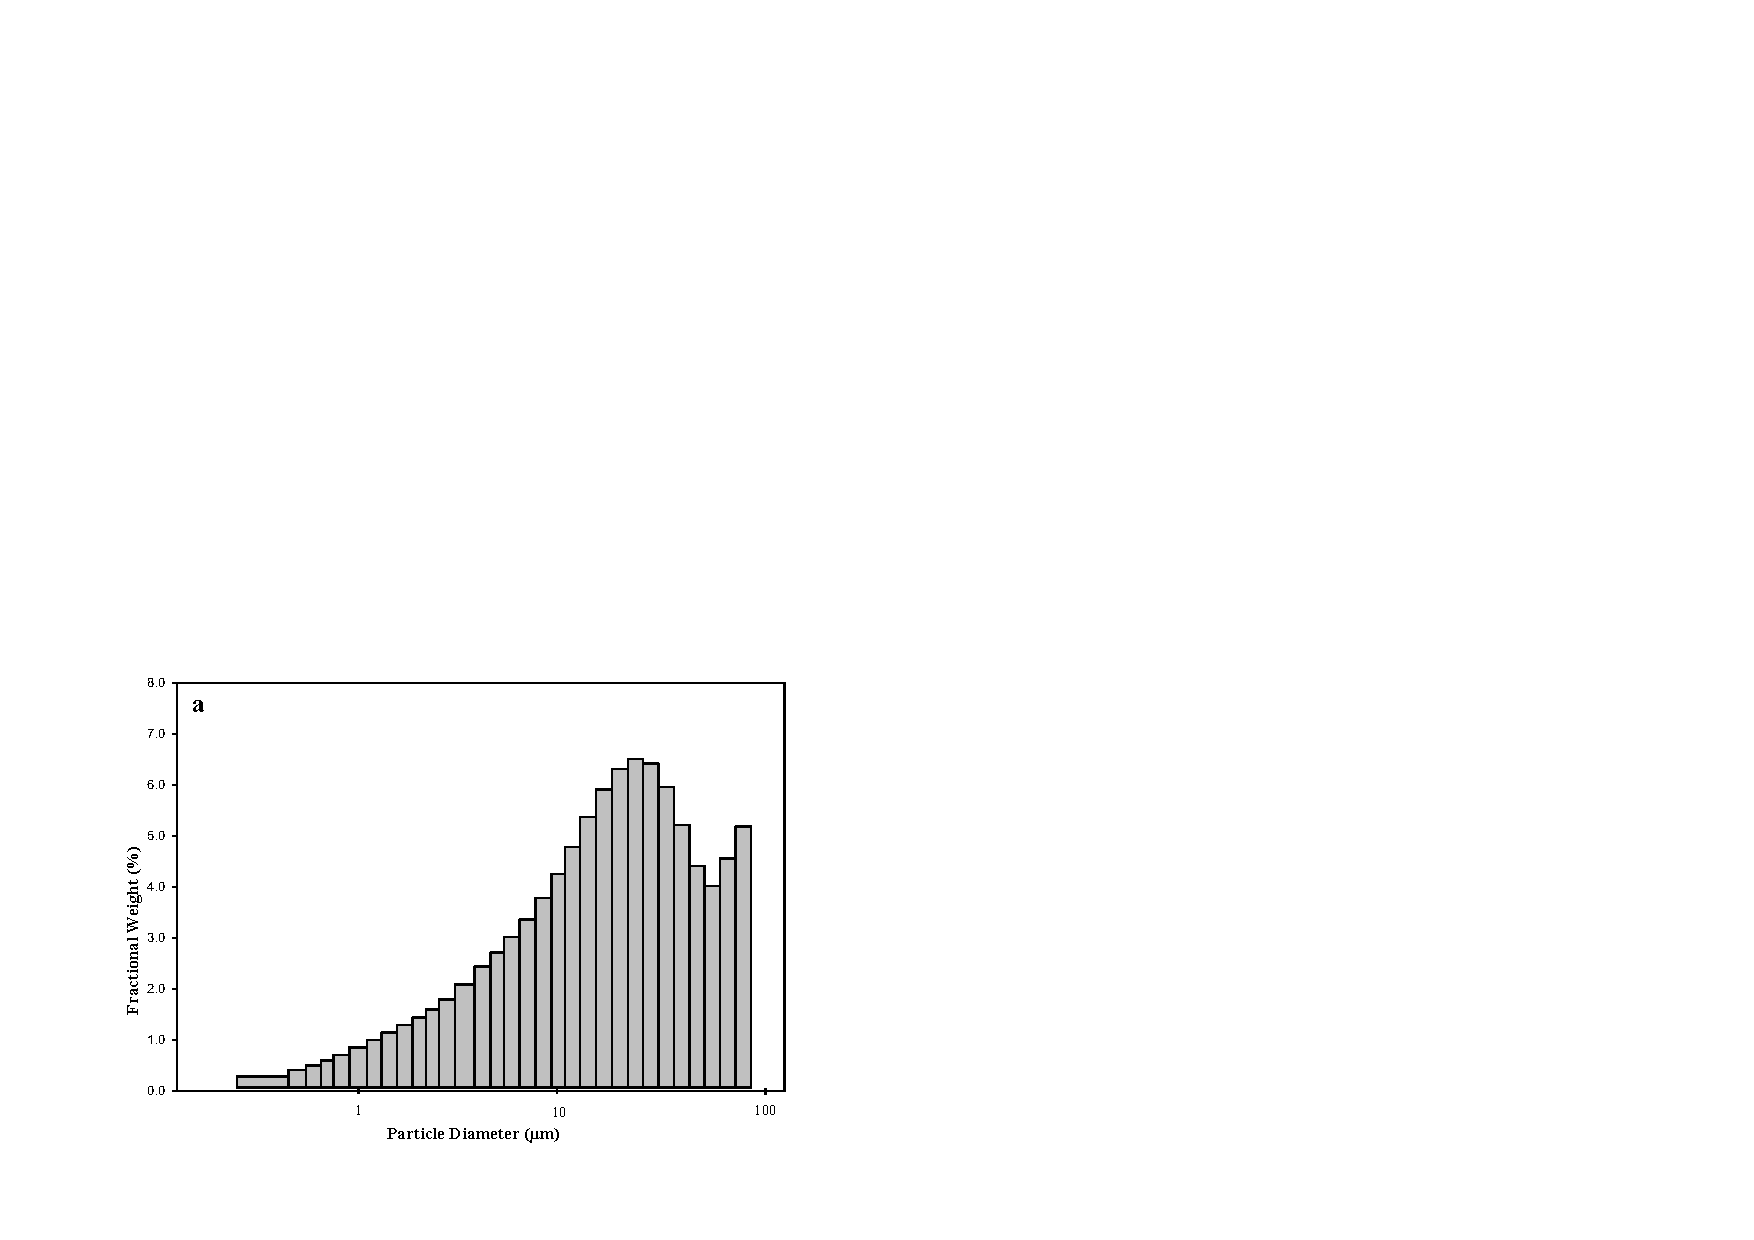
\includegraphics[height=0.6\textwidth]{finedistribution.pdf}
  \caption{}
   \label{fig:finepsd}
\end{subfigure}%
\begin{subfigure}{.5\textwidth}
  \centering
  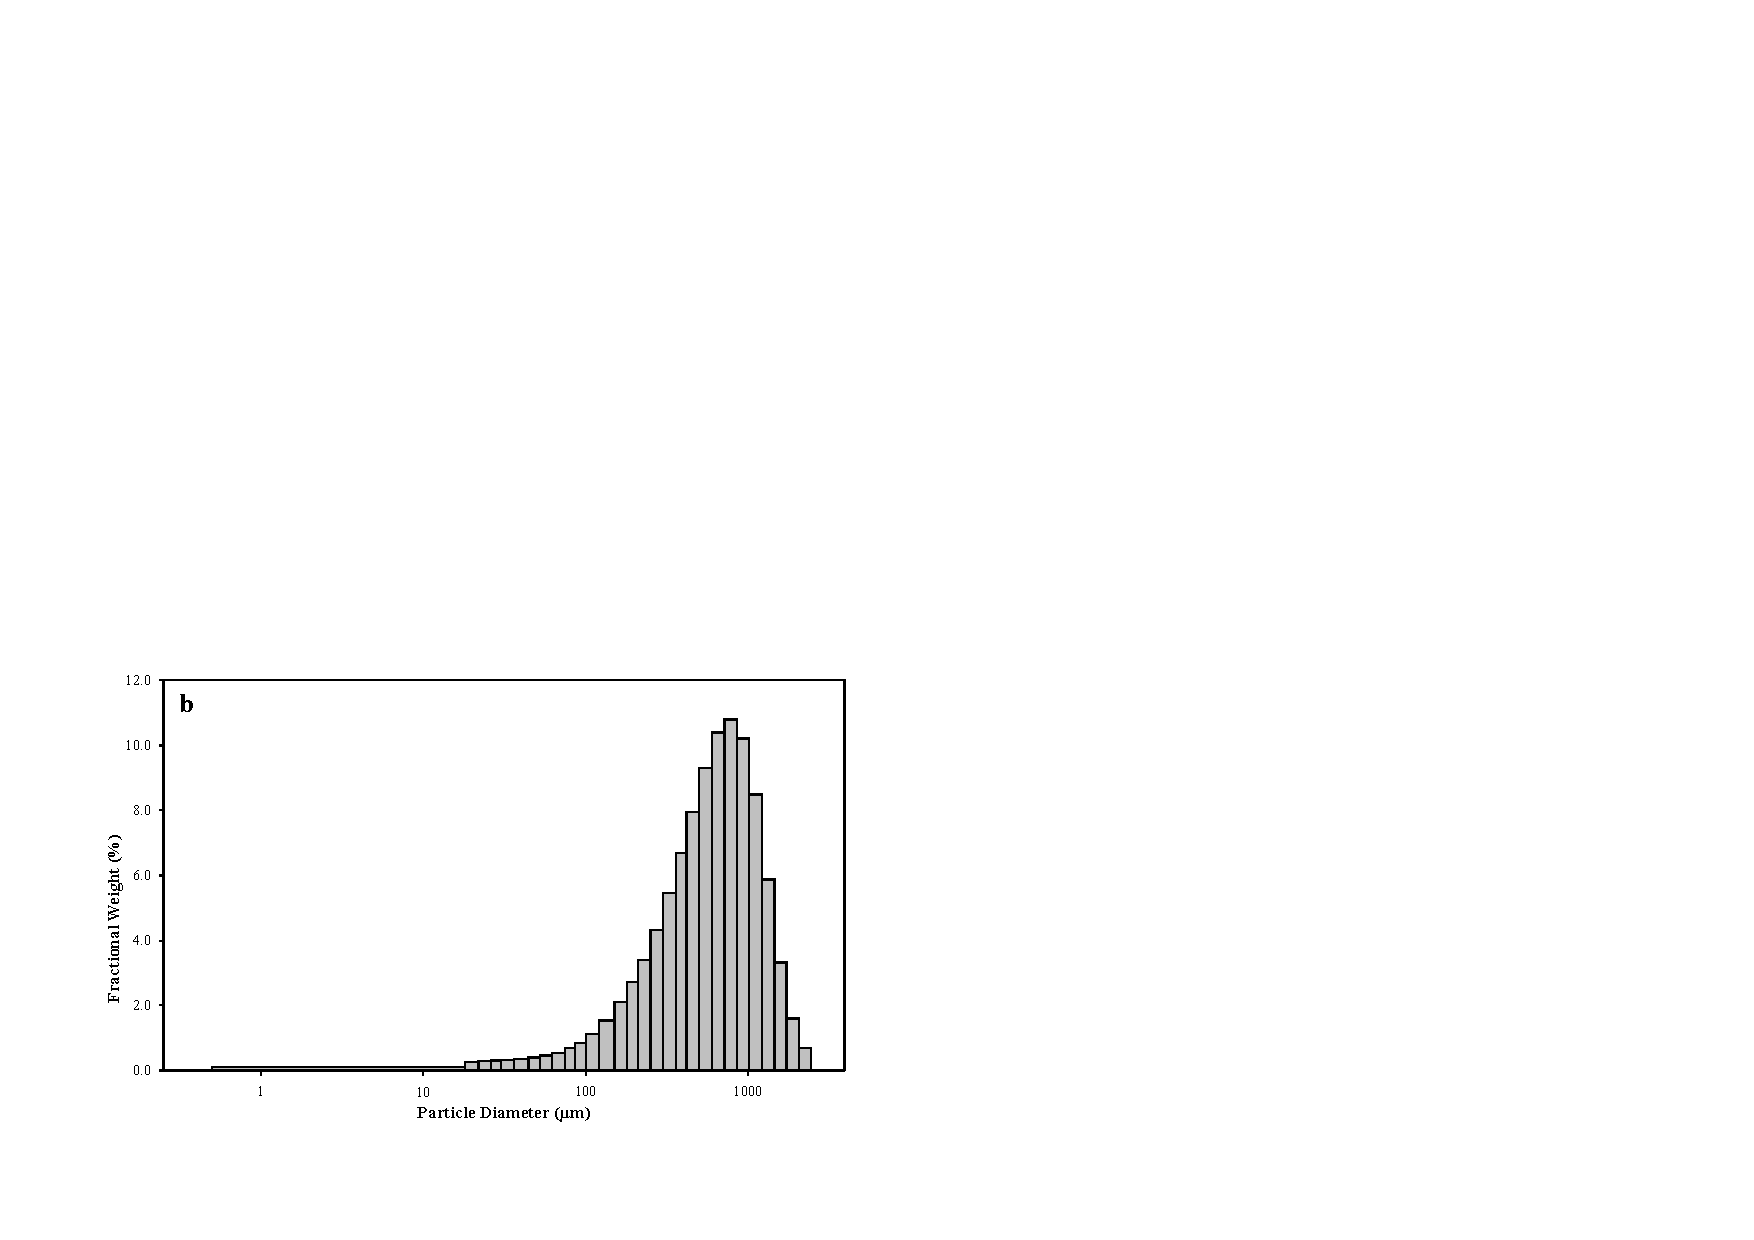
\includegraphics[height=0.62\textwidth]{coarsedistribution.pdf}
  \caption{}
    \label{fig:coarsepsd}
\end{subfigure}
\caption{Particle size distribution of fine (a) and coarse (b) grain-type particles. The fractional weight (\si{\percent}) is the fraction of olivine retained on a sieve of a particular aperture size (expressed as mean particle diameter here). Results prepared by collegues in the working group Sedimentology and Stratigraphy at the University of Hamburg}
\end{figure}
\begin{figure}[H]
\centering
  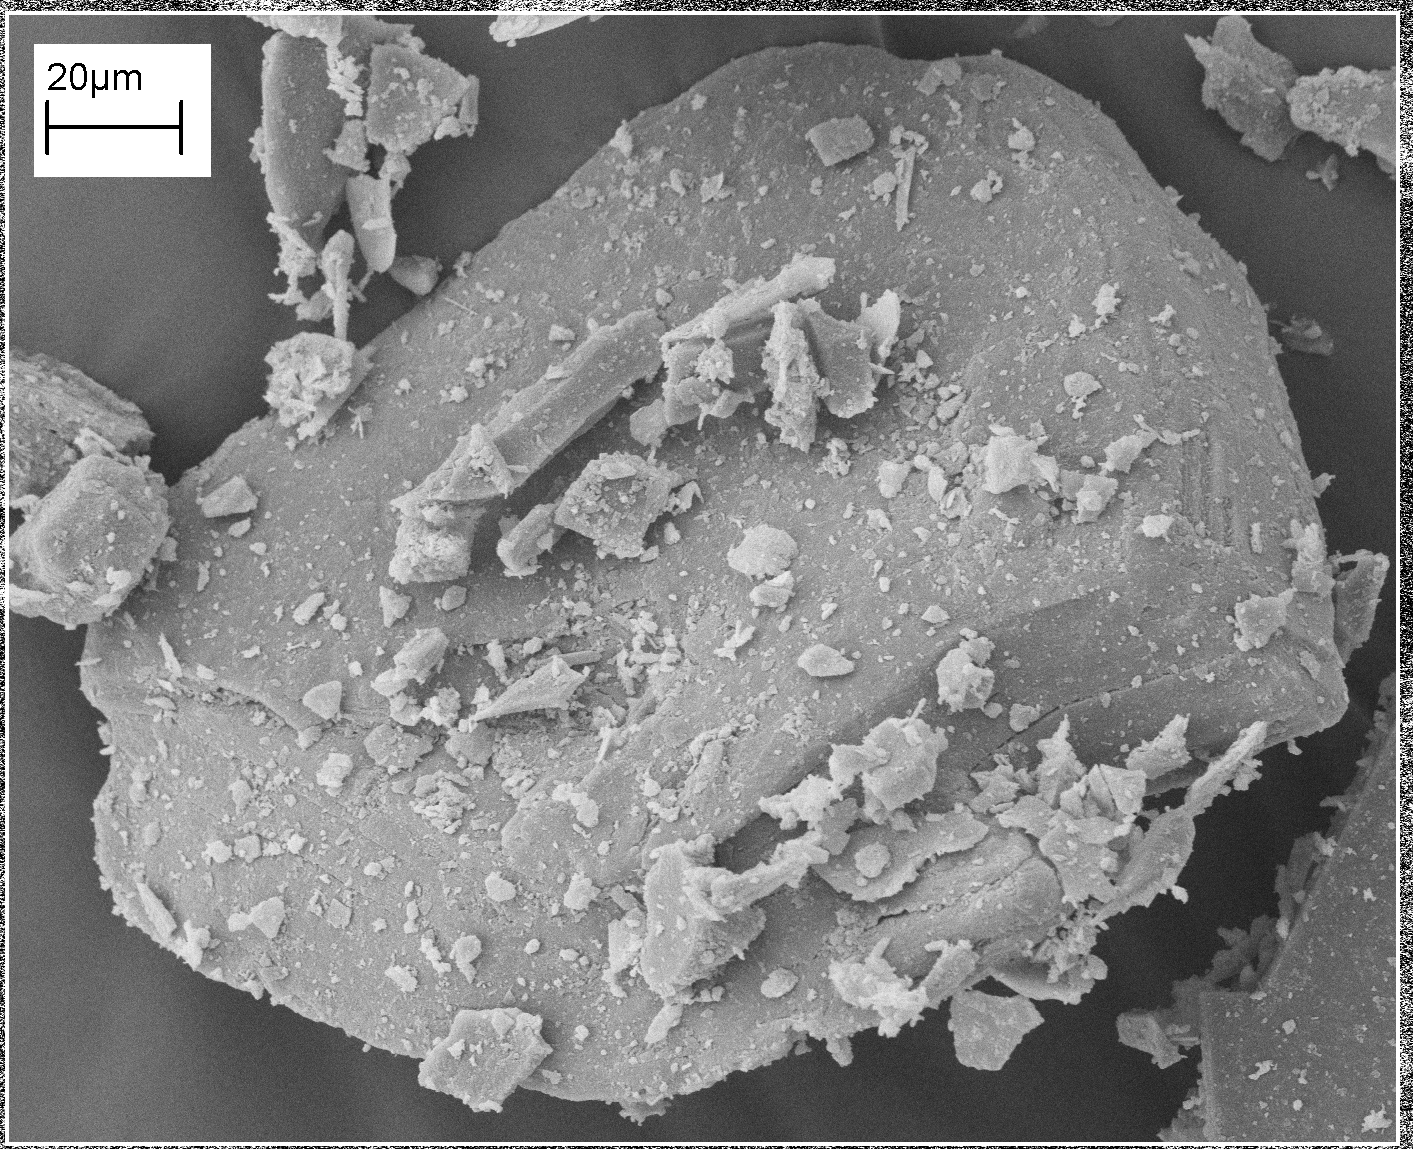
\includegraphics[scale=0.4]{SEM.png}
  \caption{Scanning electron microscope (SEM) image of an olivine grain showing a coarse particles and the many fines and ultrafines adhering to it \citep{marvin}.}
  \label{fig:SEM}
 \end{figure}
\section{Experimental setup}
The setup (see \Cref{fig:column,fig:setup}) consisted of nine acrylic cylindrical tubes with outer diameter/inner diameter/height of 60/56/250 \si{mm} respectively. A \SI{20}{\micro\meter} nylon mesh\footnote{\url{Hydro-Bios, http://www.hydrobios.de/plankton-nets/}} was fixed at the bottom of each cylinder using electrical tape. The nylon mesh allowed water to flow through but not the rock powder. Three holes were drilled at \SI{5}{cm} intervals (measured from bottom) for each cylinder, to allow insertion of Rhizons . A Rhizon\footnote{\url{Rhizosphere, http://www.rhizosphere.com/rhizons}} is a micro-filtering membrane used to extract pore water samples from soil layers or sediments.  Crushed olivine without any chemical pre-treatment was filled till \SI{20}{cm} height (measured from bottom), tapping the cylinder along the way to compress the powder. The first three cylinders contained coarse grain-type (\SIrange[range-units = single,range-phrase = --]{0}{3}{\milli\metre}), the next three fine grain-type (\SI{<63}{\micro\meter}) and the last three were a 1:1 mixture by weight of the two grain types. The weight of the olivine powder in each cylinder was subsequently measured. The total surface area (TSA) was calculated by multiplying the weight of the olvine in each column to the specific surface area measured by BET. The results are listed in \Cref{tab:physicalcharacter}. All cylinders stood upright using clamps and clamp-stands. The opening was covered with aluminum foil to decrease water loss by evaporation. Outlet/exit water was collected in plastic bottles. The setup was kept in an air-conditioned room set at \SI{25}{\degreeCelsius} but room thermometers showed variation between \SIrange[range-units = single,range-phrase = --]{22}{26}{\degreeCelsius} during the duration of the experiment.

\begin{figure}
\CenterFloatBoxes
\begin{floatrow}
\ffigbox
  {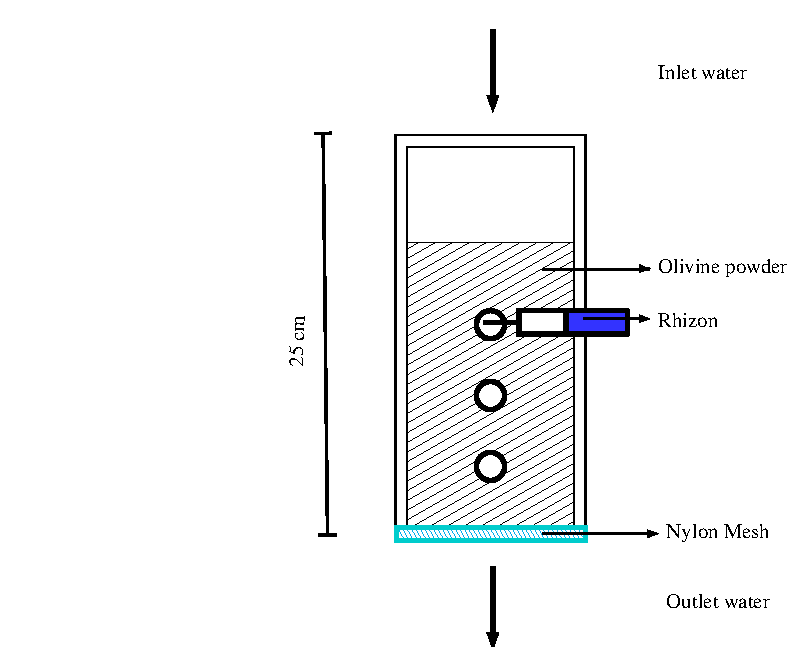
\includegraphics[scale=.75]{illustration_column.pdf}}
  {\caption{Illustration of the column design}}
  \label{fig:column}
\killfloatstyle
\ttabbox
  {\begin{tabular}{lc}
     \toprule
    \textbf{Composition} & \textbf{Mass (\%)} \\
    \midrule
    \ce{SiO_2} & 40.14 \\
   \ce{Al2O3} & 0.70 \\
   \ce{Fe_2O_3} & 6.75 \\
   \ce{MnO} & 0.09 \\
    \ce{MgO} & 44.99 \\
    \ce{CaO} & 0.40 \\
  \ce{Na2O} & 0.03 \\
    \ce{K2O} & 0.06 \\
    \ce{TiO2} & 0.01 \\
    \ce{P_2O_5} & 0.01 \\
    \text{Loss on ignition} & 6.48 \\
    \textbf{Total} & 99.68 \\
    \bottomrule
    \end{tabular}}
   {\caption{Mineral composition from XRF analysis \citep{marvin}}
   \label{tab:composition}}
\end{floatrow}
\end{figure}

The experiment started on 5 June 2015 and continues to date although data is analysed only till 14 March 2016. \SI{75}{\milli\litre} of ultrapure Milli-Q\texttrademark \;(conductivity of \SI{18}{\mega\ohm}) was added to each cylinder, five days a week. Thus, the total amount of water added (excl. weekends and holidays) was (274 $\times$ 74) \SI{20.55}{\litre}. The sampling frequency, i.e., how often water samples are collected from the outlets and rhizons changed during the experiment run. During the first four months, outlet samples were collected every day while rhizon samples were collected twice a week. The frequency was subsequently decreased, to bimonthly for both outlet and rhizons, and currently only monthly measurements are taken. 
\begin{figure}
\centering
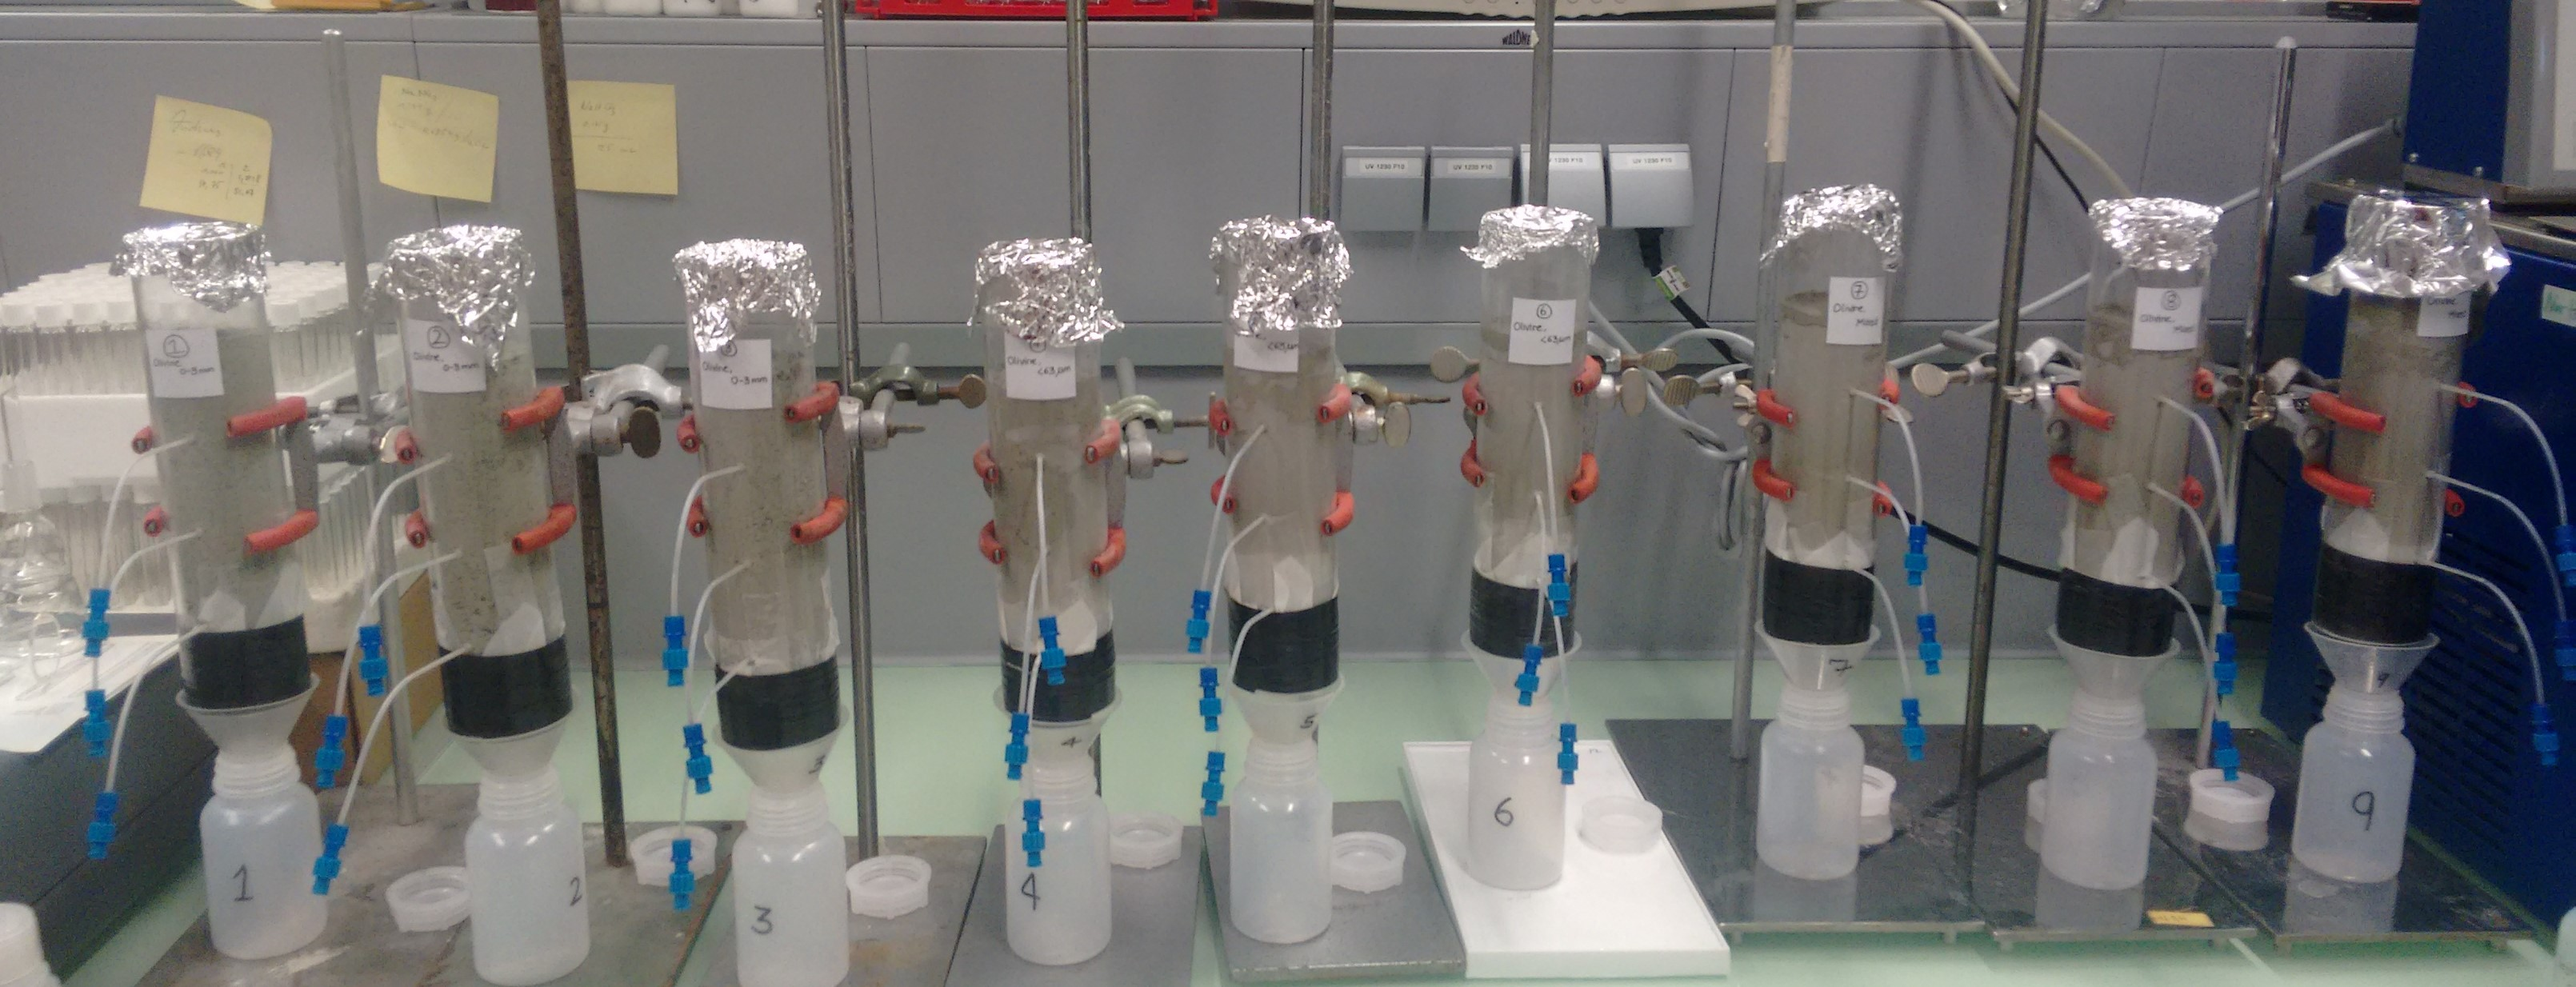
\includegraphics[width=\textwidth]{lab1.jpg}
\caption{Experimental setup showing arrangement of the columns containing olivine (\numrange{1}{3} are coarse, \numrange{4}{6} are fine, and \numrange{7}{9} are mixed), rhizones to collect pore water, and containers to collect outlet water.}
\label{fig:setup}
\end{figure}

\begin{table}[h]
  \centering
      \begin{tabular}{clll}
    \toprule
    \textbf{Column} & \textbf{Grain-type} & \textbf{Weight  (\si{\gram})} & \textbf{TSA (\si{m^2})} \\
    \midrule
    1     & coarse & 961.0 & 1018.66 \\
    2     & coarse & 984.3 & 1043.36 \\
    3     & coarse & 1003.6 & 1063.82 \\
    4     & fine  & 630.3 & 6006.76 \\
    5     & fine  & 676.1 & 6443.23 \\
    6     & fine  & 660.0 & 6289.80 \\
    7     & mixed & 913.3 & 4835.92 \\
    8     & mixed & 881.3 & 4666.48 \\
    9     & mixed & 908.8 & 4812.10 \\
    \bottomrule
    \end{tabular}
   \caption{Physical characterisation of olivine in the columns with column number, grain-type, weight and total surface area (TSA)}
  \label{tab:physicalcharacter}
\end{table}

\section{Solution analysis}
The outlet samples were measured for pH, total alkalinity, dissolved silica, and major ion composition. Total alkalinity was measured using a Metrohm Titrando 818\texttrademark\ up to a pH endpoint of \num{4.3}. The Si concentration is measured as dissolved silica \ce{Si(OH)_4} and measured using the molybdate blue colometric method. The major ion composition was determined using a Metrohm\texttrademark\ Ion Chromatograph (IC) using a column that could identify \ce{Ca^{+2}}, \ce{K+}, \ce{Mg^{+2}}, \ce{Na+},\ce{SO^{-2}_4}, \ce{NO^-_3}. All the concentrations were reported in \si{\micro\mole\per\litre}. The pH was measured using a WTW\texttrademark\ hand-held pH meter calibrated with three points using NIST buffer standards.